\chapter{Technical Background}
\label{capitulo3}

In this chapter an overview about the main concepts of this work will be described. The present section is divided in three major sections. In Section \ref{sensors}, the concepts of sensors is defined. In Section \ref{image-processing} covers the technical background about image processing. In Section \ref{ml-ai}, the main concepts regarding machine learning and artificial intelligence are described. In Section \ref{autonomous-vehicles} is defined the major concepts about autonomous vehicles.

\section{Sensors}\label{sensors}

It is possible to have more sensors in autonomous vehicles, but these three sensors are the main in Autonomous vehicles structure. As is positioned in the Figure \ref{fig:autonomous-vehicles} the correct place for the most important sensors.


\begin{figure}[H]
\centering
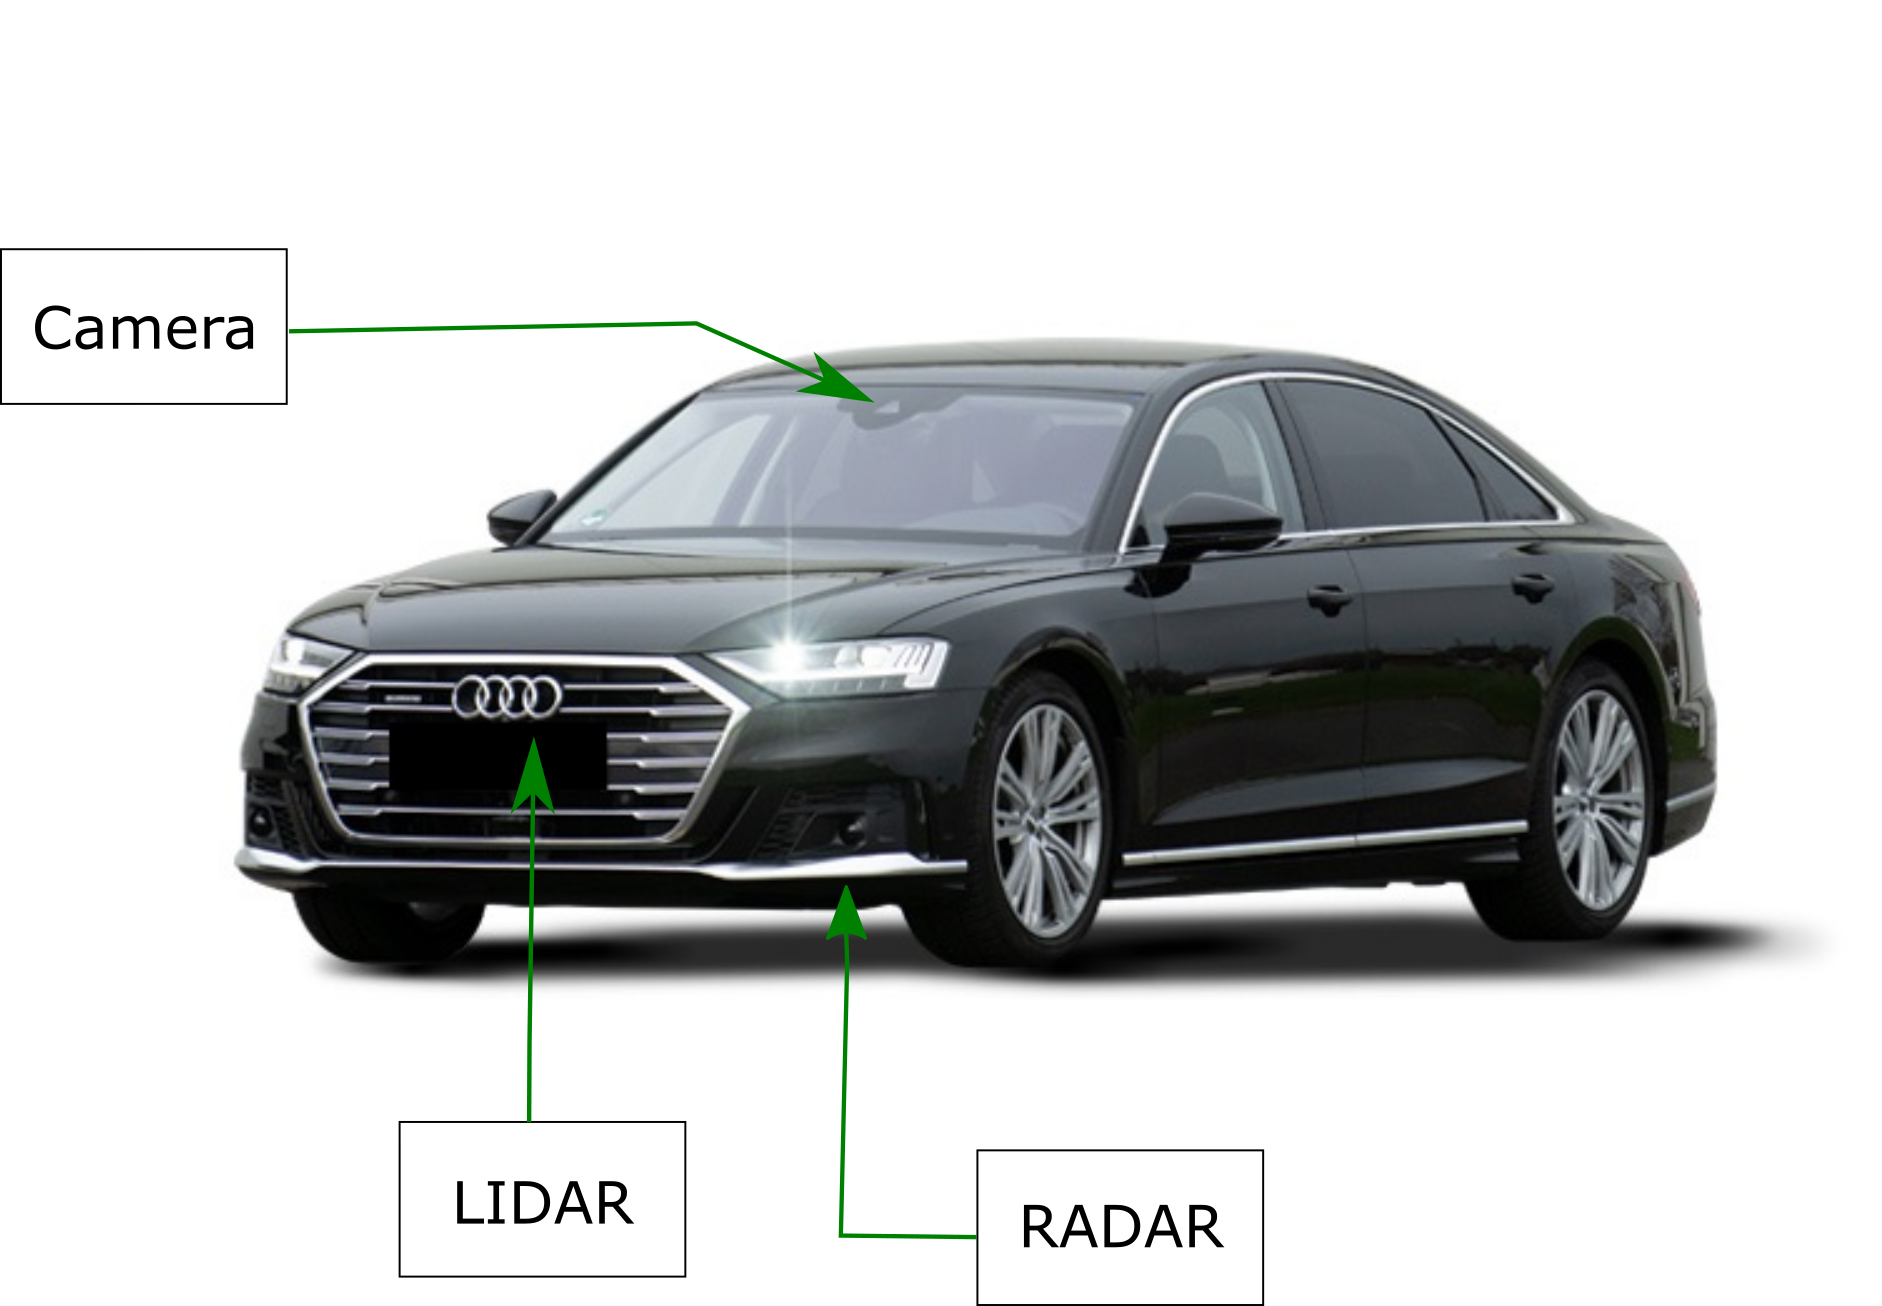
\includegraphics[scale=0.7]{imagens/image823.png}
\caption{Representation of an autonomous vehicle}
\label{fig:autonomous-vehicles}
\end{figure}


\subsection{Camera}
The camera is a kind of sensor whose allows the car to see the environment using the collected image, in Figure \ref{fig:camera} is shown the standard camera for autonomous vehicles. 

\begin{figure}[H]
\centering
\includegraphics[width=\columnwidth]{imagens/camera.png}
\caption{Representation of a camera of the autonomous vehicle}
\label{fig:camera}
\end{figure}

\subsection{Radar}
\subsection{Lidar}
The lidar is a kind of sensor whose allows the car to see the environment using the collected image, in Figure \ref{fig:lidar} is shown the standard camera for autonomous vehicles. 

\begin{figure}[H]
\centering
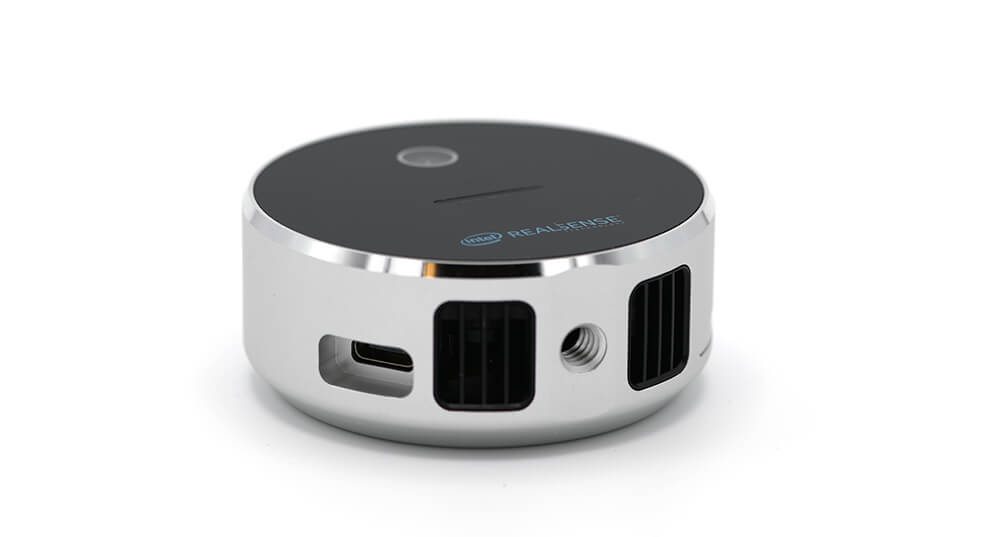
\includegraphics[width=\columnwidth]{imagens/lidar.jpg}
\caption{An exemple of a lidar of the autonomous vehicle}
\label{fig:lidar}
\end{figure}

\section{Machine Learning}\label{ml-ai}
The machine learning is approach based on algorithms to create some predictions, these techniques are based on mathematical and computer science, it is possible to apply this in several fields of the science. 
\subsection{Artificial Neural Networks}

The artificial neural networks (ANN) or percpetron were inspired in the human brain. This approach is because the capacity of the human brain to categorize new information. In Figure \ref{fig:ann} is shown an example of the structure of an ANN. Where there is an input array with the processed features for categorization. The next step of the processing is to define the weights for this analysis. The activation function is the main part of this process, because in this step the algorithm will transform the numbers collect by the previous steps and will return only in binary purpose, like $0$ and $1$ in the output layer \cite{goodfellow2016deep}.

\begin{figure}[H]
\centering
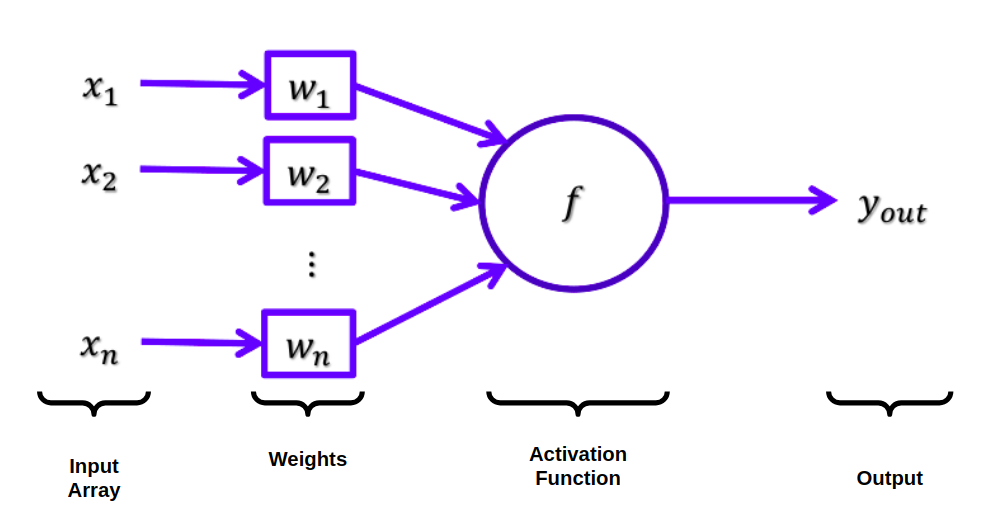
\includegraphics[width=\columnwidth]{imagens/ann.png}
\caption{The structure of an ANN}
\label{fig:ann}
\end{figure}

So, mathematically, the neuron output is a function of weighted sum of its inputs. Figure \ref{fig:ann_weight} is shown the mathematical background. Where $f$ is activation function, $w_i$ are the weights, and $\beta$ is the constant input called as bias.


\begin{figure}[H]
\centering
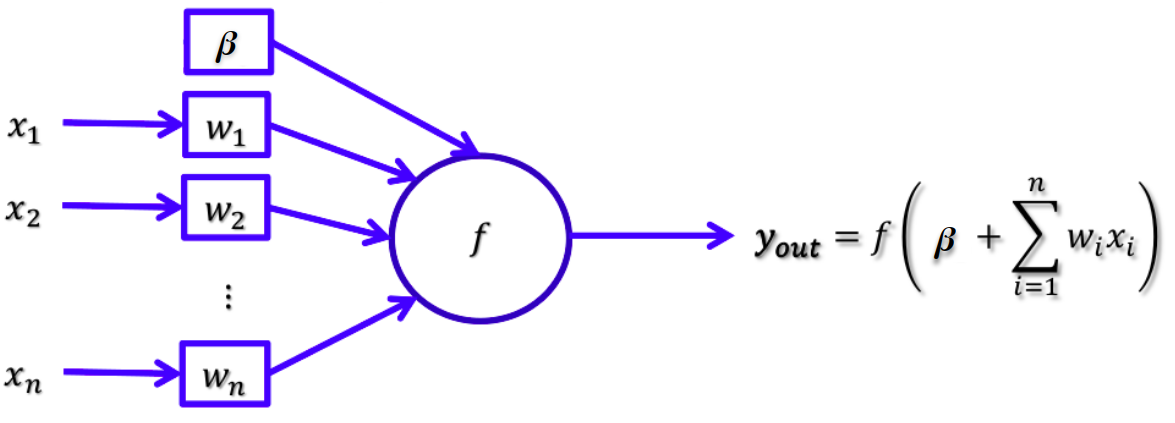
\includegraphics[width=\columnwidth]{imagens/math_ann_bias.png}
\caption{Mathematical representation of ANN with bias}
\label{fig:ann_weight}
\end{figure}


\subsubsection{Activation functions}
There are many different activation functions to use. These are crucial for the ANN characteristics, such as learning ability and computational efforts in terms of training and validation.

\begin{itemize}
    \item Unit step function
    \item Sign function
    \item Identity function
    \item Sigmoid function
    \item Hyperbolic tangent function
    \item Retified linear unit (Relu) 
\end{itemize}

\begin{table}[H]
\label{tab:tab1} 
\caption{Comparison Table for Activation Functions}
\centering
\resizebox{15.3cm}{!}{%
\begin{tabular}{|c|c|c|c|c|c|c|}
\hline
\textbf{\begin{tabular}[c]{@{}c@{}}Activation\\ Function\end{tabular}}  & \textbf{Linear}          & \textbf{Monotonic} & \textbf{Continuous}      & \textbf{\begin{tabular}[c]{@{}c@{}}Derivative \\ Monotonic\end{tabular}} & \textbf{\begin{tabular}[c]{@{}c@{}}Derivative\\ Continuous\end{tabular}} & \textbf{\begin{tabular}[c]{@{}c@{}}Simetric with \\ respect to \\ The Origin\end{tabular}} \\ \hline
{\color[HTML]{000000} Unit Step} & {\color[HTML]{FE0000} x} & {\color[HTML]{009901} \checkmark}& {\color[HTML]{FE0000} x} & {\color[HTML]{FE0000} x} & {\color[HTML]{FE0000} x} & {\color[HTML]{FE0000} x} \\ \hline
Sign & {\color[HTML]{FE0000} x} & {\color[HTML]{009901} \checkmark}& {\color[HTML]{FE0000} x} & {\color[HTML]{FE0000} x} & {\color[HTML]{FE0000} x} & {\color[HTML]{009901} \checkmark} \\ \hline
Identity & {\color[HTML]{009901} \checkmark}& {\color[HTML]{009901} \checkmark}& {\color[HTML]{009901} \checkmark}& {\color[HTML]{FE0000} x} & {\color[HTML]{009901} \checkmark}& {\color[HTML]{009901} \checkmark}\\ \hline
Sigmoid                                                                 & {\color[HTML]{FE0000} x} & {\color[HTML]{009901} \checkmark}             & {\color[HTML]{009901} \checkmark}                   & {\color[HTML]{FE0000} x}                                                 & {\color[HTML]{009901} \checkmark}                                                                   & {\color[HTML]{FE0000} x}                                                               \\ \hline
\begin{tabular}[c]{@{}c@{}}Hyperbolic\\ Tangent\end{tabular}            & {\color[HTML]{FE0000} x} & {\color[HTML]{009901} \checkmark}             & {\color[HTML]{009901} \checkmark}                   & {\color[HTML]{FE0000} x}                                                 & {\color[HTML]{009901} \checkmark}                                                                   & {\color[HTML]{009901} \checkmark}                                                                                 \\ \hline
\begin{tabular}[c]{@{}c@{}}Rectified \\ Linear Unit \\ (ReLU)\end{tabular} & {\color[HTML]{FE0000} x} & {\color[HTML]{009901} \checkmark}              & {\color[HTML]{009901} \checkmark}                   & {\color[HTML]{009901} \checkmark}                                                                   & \begin{tabular}[c]{@{}c@{}}{\color[HTML]{FE0000} x}\\ (at 0)\end{tabular}                       & {\color[HTML]{FE0000} x}                                                               \\ \hline
\end{tabular}}
\end{table}

In this work, Relu is the activation function chosen activation. Its mathematical definition is show in (\ref{eq:relu}). 


\begin{equation}
\label{eq:relu}
    f(x) = \mathrm{R}(x) = \mathrm{max}(0,x)
\end{equation}


The graphic visualization of the function Relu is shown in Figure \ref{fig:relu}, where this function return $0$ if the number from the weighted sum is below than $0$, or return $x$ if the previous value is over than $0$.


\begin{figure}[H]
\centering
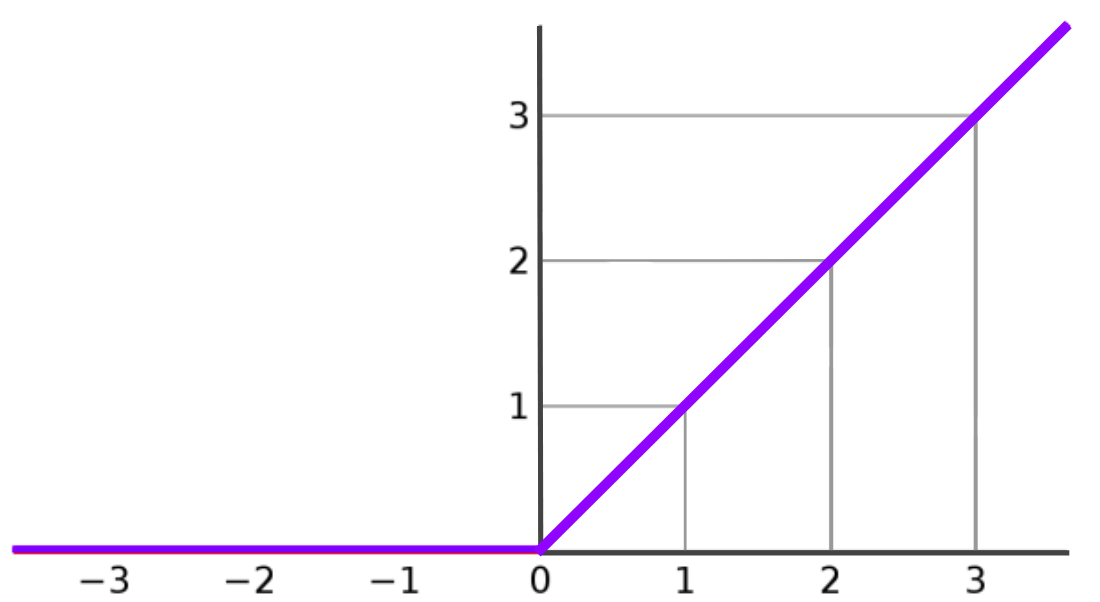
\includegraphics[scale=0.3]{imagens/relu_corrected.png}
\caption{The behavior of the Relu}
\label{fig:relu}
\end{figure} 

These are the important characteristics of this activation function.

    \begin{itemize}
        \item Widely used in deep networks
        \item Pros: nonlinear, monotonic, derivative monotonic, and fast convergence
        \item Cons: not continuously differentiable at zero, i.e. issues with gradient descent around origin.
    \end{itemize}

\subsubsection{Layered Neural Networks}

The quint essential example of a deep learning model is the multilayer perceptron (MLP). A MLP is just a mathematical function mapping some set of input values to output values. The function
is formed by composing many simpler functions \cite{goodfellow2016deep}.


These are the quint essential deep learning models. The goal
of a feedforward network is to approximate some function $f*$. For example, for a classifier, $y = f*(x)$ maps an input x to a category y. A feedforward network
defines a mapping $y = f (x; \theta)$ and learns the value of the parameters $\theta$ that resultin the best function approximation.

These models are called feedforward because information flows through the function being evaluated from $x$, through the intermediate computations used to define $f$, and finally to the output $y$. There are no feedback connections in which outputs of the model are fed back into itself.



\subsection{Convolutional Neural Networks}


The Convolutional Neural Networks (CNN) are a specialized kind of neural network for processing data that has a known \cite{lecun1995convolutional}. For example in autonomous vehicles domain, this approach is several used for object detection and object identification. This name  indicates that the network employs a mathematical operation called
convolution. 

A CNN coarsely scans the image for features (in lower dimension space), pools possible patterns, then inspect those patterns in detail with its fully connected
subnetworks, generating their classifications. In Figure \ref{fig:cnn_car} is defined the full process of this neural network. Where there are three other importants is steps: Convolutional layer is defined in Subsection \ref{sub:conv}. The pooling layer is introduced in the Subsection \ref{sub:pooling}. The fully connected layers is introduced in Subsection \ref{sub:fully}.

\begin{figure}[H]
\centering
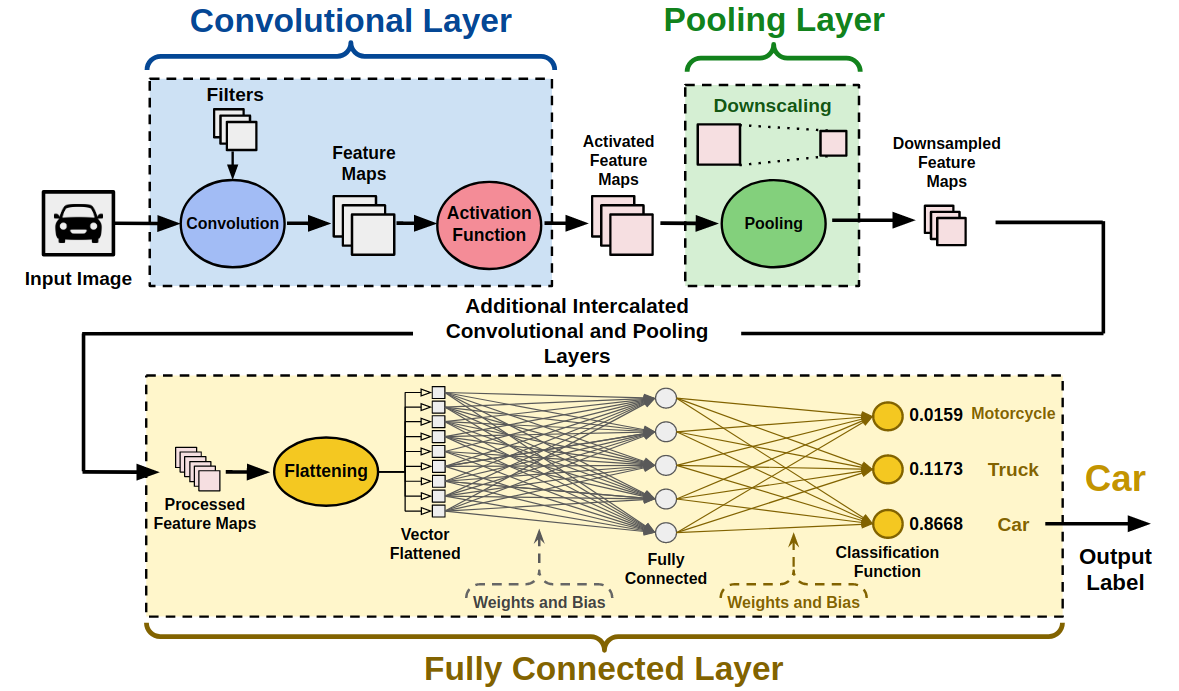
\includegraphics[width=\columnwidth]{imagens/Full_Process.png}
\caption{Full process of a convolutional neural network}
\label{fig:cnn_car}
\end{figure}


\subsubsection{Convolutional Layer}
\label{sub:conv}

When the convolutional layer is introduced, common inputs are tridimensional matrix with height and width defined accordingly with the image dimensions and determined by the amount of colors. In general the images use three color channels, Red-Green-Blue (RGB) as is shown in Figure \ref{fig:rgb}.

\begin{figure}[H]
\centering
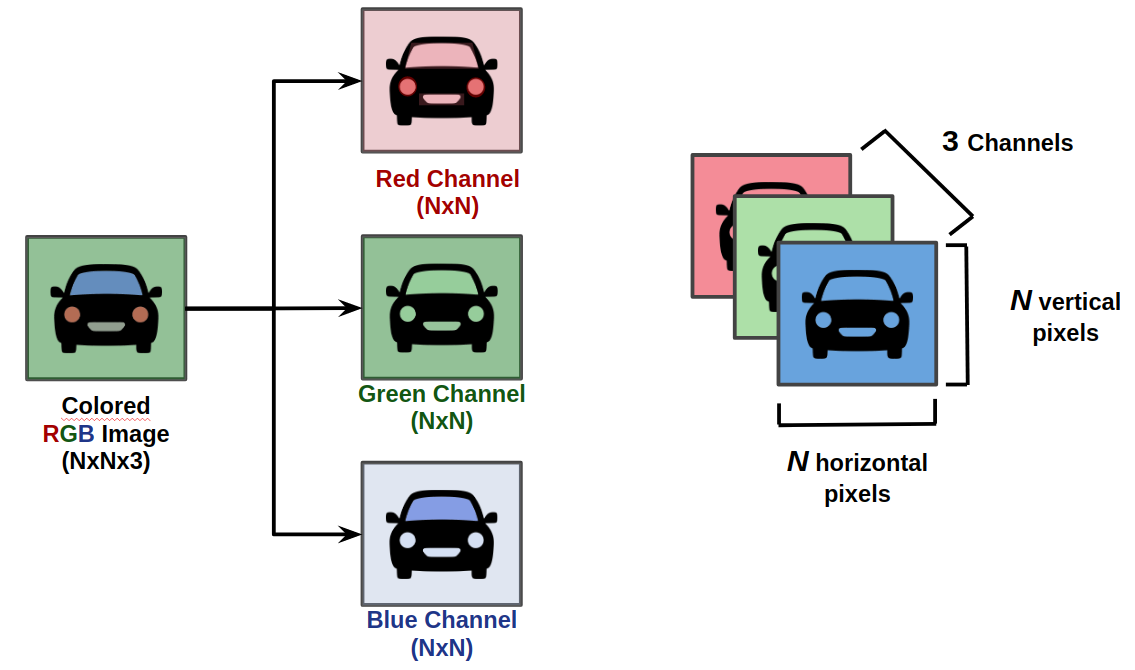
\includegraphics[scale=0.35]{imagens/rgb_representation.png}
\caption{Representation of the colors of the input image}
\label{fig:rgb}
\end{figure}


The convolutions work as filters that seem little squares and they are slipping through whole image and capturing the most important parts. For example in Figure \ref{fig:bias}, an image with $NxNX3$ and a filter with the $MxMX3$, where the main different is that each result is then summed, along with the Bias ($\beta$) value, to be then passed to the activation function. And in the end of the process generates a new matrix called as feature map or activation map.


\begin{figure}[H]
\centering
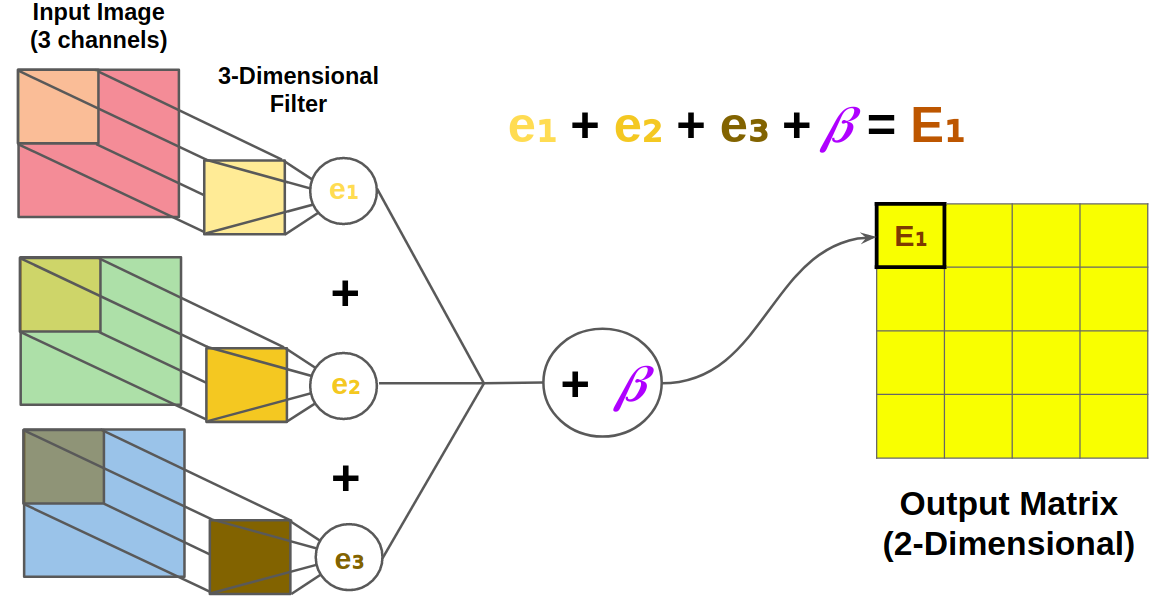
\includegraphics[scale=0.35]{imagens/three_dim_conv_2.png}
\caption{Representation of the convolution process}
\label{fig:bias}
\end{figure}




\subsubsection{Pooling and Upsampling}\label{sub:pooling}

A pooling layer is necessary to simplify the information from the previous layer. As happens with the convolution layer, it is choose an unit area, for example $2x2$ to slicing for the whole output information from the previous step. To brief, if the information from the previous layer was $4x4$, the output from process of pooling will be $2x2$. Nevertheless, the most used method is maxpooling, where the biggest number in the matrix is passed to the next step, this data summarization is used to reduce the amount of weights and to avoid overfitting. In Figure \ref{fig:pooling} is shown the maxpooling process.

\begin{figure}[H]
\centering
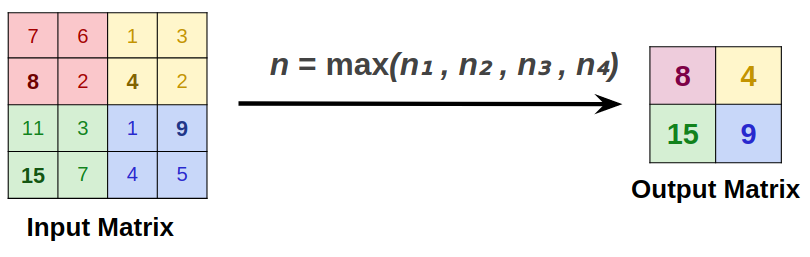
\includegraphics[scale=0.35]{imagens/max_pooling.png}
\caption{Representation of the maxpooling process}
\label{fig:bias}
\end{figure}




\subsubsection{Auto-encoders}
\subsubsection{Training}
\subsubsection{Losses}
\subsubsection{Stochastic Gradient Descent}
\subsubsection{Weight Initialization}
\subsubsection{Error Backpropagation}

\subsubsection{Fully Connected Layers}\label{sub:fully}
\subsubsection{Regularization}
\subsubsection{Data Augmentation}



\section{Autonomous Vehicles} \label{autonomous-vehicles}
\subsection{What are autonomous vehicles}
\subsection{History and current research}
\subsection{Challenges}
\subsection{Levels	of	Automation}
\subsection{Effects of autonomous vehicles in the society}